\documentclass[psamsfonts]{amsart}

%-------Packages---------
\usepackage{amssymb,amsfonts}
\usepackage{semantic}
\usepackage{fullpage}
\usepackage{tikz-cd}
\usepackage{todonotes}
\usepackage{physics}
\usepackage[all,arc]{xy}
\usepackage{enumerate}
\usepackage{enumitem}
\usepackage{mathrsfs}
\usepackage{theoremref}
\usepackage{graphicx}
\usepackage[bookmarks]{hyperref}

%--------Theorem Environments--------
%theoremstyle{plain} --- default
\newtheorem{thm}{Theorem}[section]
\newtheorem{cor}[thm]{Corollary}
\newtheorem{prop}[thm]{Proposition}
\newtheorem{lem}[thm]{Lemma}
\newtheorem{conj}[thm]{Conjecture}
\newtheorem{quest}[thm]{Question}

\theoremstyle{definition}
\newtheorem{defn}[thm]{Definition}
\newtheorem{defns}[thm]{Definitions}
\newtheorem{con}[thm]{Construction}
\newtheorem{exmp}[thm]{Example}
\newtheorem{exmps}[thm]{Examples}
\newtheorem{notn}[thm]{Notation}
\newtheorem{notns}[thm]{Notations}
\newtheorem{addm}[thm]{Addendum}
\newtheorem{exer}[thm]{Exercise}
\newtheorem{innercustomexer}{Exercise}
\newenvironment{customexer}[1]
  {\renewcommand\theinnercustomexer{#1}\innercustomexer}
  {\endinnercustomexer}

\theoremstyle{remark}
\newtheorem{rem}[thm]{Remark}
\newtheorem{rems}[thm]{Remarks}
\newtheorem{warn}[thm]{Warning}
\newtheorem{sch}[thm]{Scholium}

\DeclareMathOperator{\Hom}{Hom}
\DeclareMathOperator{\Id}{Id}
\DeclareMathOperator{\End}{End}
\DeclareMathOperator{\ord}{ord}
\DeclareMathOperator{\Aut}{Aut}
\DeclareMathOperator{\Gal}{Gal}
\DeclareMathOperator{\RP}{\mathbb{R}\mathbb{P}}
\DeclareMathOperator{\Int}{Int}

\makeatletter
\let\c@equation\c@thm
\makeatother
\numberwithin{equation}{section}

\bibliographystyle{plain}

\begin{document}

\title{Introduction to Smooth Manifolds}
\author{Hidenori Shinohara}

\maketitle
\tableofcontents

\section{Chapter 1}
\subsection{Exercises}
\begin{customexer}{1.1}\label{exercise_1_1}
  Show that equivalent definitions of manifolds are obtained if instead of allowing $U$ to be homeomorphic to \textit{any} open subset of $\mathbb{R}^n$, we require it to be homeomorphic to an open ball in $\mathbb{R}^n$, or to $\mathbb{R}^n$ itself.
\end{customexer}

\begin{proof}
  It is clear that a ``manifold" satisfying the open-ball or $\mathbb{R}^n$ definition satisfies the open-subset definition.
  Let $M$ be a manifold satisfying the open-subset definition.
  Let $x \in M$ be given and let $U, \hat{U}, \phi$ be given according to the definition.
  Since $\hat{U}$ is open, there exists an open ball $B$ such that $\phi(x) \in B \subset \hat{U}$.
  Restrict $\phi$ to $\phi^{-1}(B)$.
  Then $\phi^{-1}(B)$ is an open subset of $M$ containing $x$, and $\phi\mid_{\phi^{-1}(B)}$ is a homeomorphism between $\phi^{-1}(B)$ and $B$.
  Thus $M$ satisfies the open-ball definition.

  $B(x, r) \subset \mathbb{R}^n$ is homeomorphic to $\mathbb{R}^n$ by the map $(x_1 + a_1, \cdots, x_n + a_n) \mapsto (\frac{a_1}{r - a_1}, \cdots, \frac{a_n}{r - a_n})$ where $x = (x_1, \cdots, x_n)$ is the center of $B(x, r)$ and $r$ is the radius.
  Since the composition of two homeomorphisms gives a homeomorphism, $M$ also satisfies the $\mathbb{R}^n$ definition as well.
\end{proof}


\begin{customexer}{1.6}
  Show that $\RP^n$ is Hausdorff and second-countable, and is therefore a topological $n$-manifold.
\end{customexer}

\begin{proof}
  From the definition of $\pi$, it is easy to see that $\pi(B(x, r))$ is open in $\RP^n$ where $x \in S^n$ and $0 < r < 1$.

  Let $[x], [y] \in \RP^n$ be given.
  Without loss of generality, assume $x, y \in S^{n}$.
  Let $r = \min\{ \abs{x - y}, \abs{x + y}, 1 \} / 2$.
  Then $U_x = \pi(B(x, r)), U_y = \pi(B(y, r))$ contain $[x], [y]$, respectively.
  $\pi^{-1}(U_x), \pi^{-1}(U_y)$ are both open in $\mathbb{R}^{n + 1} \setminus \{ 0 \}$ which can be seen easily by writing down exactly which points belong to them, so $U_x, U_y$ are both open in $\RP^n$.
  Then $\pi^{-1}(U_x \cap U_y) = \pi^{-1}(U_x) \cap \pi^{-1}(U_y) = \emptyset$, so $U_x \cap U_y = \emptyset$.
  Therefore, $\RP^n$ is Hausdorff.

  Let $\mathcal{B} = \{ \pi(B(x, 1 / k)) \mid x \in \mathbb{Q}^{n + 1} \cap S^{n}, k \in \{ 2, 3, 4, \cdots \} \}$.
  Then $\mathcal{B}$ is a countable collection of open sets whose union is $\RP^n$.
  Let $U \subset \RP^n$ be a nonempty open set.
  Let $[x] \in U$.
  Since $\pi$ is a quotient map, $\pi^{-1}(U)$ is open.
  Moreover, $x \in \pi^{-1}(U)$.
  Without loss of generality, $x \in S^{n}$.
  Then $x \in B(x', 1 / k) \subset \pi^{-1}(U)$ for some $B(x', 1 / k) \in \mathcal{B}$.
  Then $[x] = \pi(x) \in \pi(B(x', 1 / k)) \subset \pi(\pi^{-1}(U)) = U$.
  Therefore, $\mathcal{B}$ is a countable basis of $\RP^n$.
\end{proof}

\begin{customexer}{1.7}
  Show that $\RP^n$ is compact.
\end{customexer}

\begin{proof}
  $\pi(S^n) = \RP^n$ and $S^n$ is compact because it is a closed, bounded subset of $\mathbb{R}^{n + 1}$. (Heine-Borel)
  Moreover, the image of a compact set under a continuous map is compact. (See A.45(a))
  Thus $\RP^n$ is compact.
\end{proof}

\begin{customexer}{1.14}
  Suppose $\mathcal{X}$ is a locally finite collection of subsets of a topological space $M$.
  \begin{enumerate}[label=(\alph*)]
    \item 
      The collection $\{ \overline{X} : X \in \mathcal{X} \}$ is also locally finite.
    \item
      $\overline{\bigcup_{X \in \mathcal{X}} X} = \bigcup_{X \in \mathcal{X}} \overline{X}$.
  \end{enumerate}
\end{customexer}

\begin{proof}
  $ $
  \begin{enumerate}[label=(\alph*)]
    \item
      Let $p \in M$.
      Then there exists an open set $U$ containing $x$ such that there are only finitely many $X \in \mathcal{X}$ such that $U \cap X \ne \emptyset$.
      Let $X \in \mathcal{X}$.
      \begin{itemize}
        \item
          If $U \cap X \ne \emptyset$, then $U \cap \overline{X} \supset U \cap X \ne \emptyset$.
        \item
          If $U \cap X = \emptyset$, then $U^c$ is closed, so $\overline{X} \subset U^c$.
          In other words, $U \cap \overline{X} = \emptyset$.
      \end{itemize}
      This shows that the number of $X \in \mathcal{X}$ that intersects $U$ and the number of $\overline{X} \in \mathcal{X}$ that intersects $U$ are the same.
      Therefore, $\{ \overline{X} : X \in \mathcal{X} \}$ is also locally finite.
    \item
      Since the closure of a set is defined to be the intersection of all closed sets containing it, $\bigcup_{X \in \mathcal{X}} \overline{X} \subset \overline{\bigcup_{X \in \mathcal{X}} X}$.
      Let $x \notin \bigcup_{X \in \mathcal{X}} \overline{X}$.
      Then there exists a neighborhood $U$ of $x$ such that $U$ intersects only finitely many $X \in \mathcal{X}$.
      Let $X_1, \cdots, X_n$ denote them.  By the same argument as part (a), $\overline{X_1}, \cdots, \overline{X_n}$ are the only elements in $\{ \overline{X} \mid X \in \mathcal{X} \}$ that $U$ intersects.
      Since $x \notin \overline{X_i}$ for each $i = 1, \cdots, n$, $U^c \cup \overline{X_1} \cup \cdots \cup \overline{X_n}$ is a closed set which contains all $X \in \mathcal{X}$ but does not contain $x$.
      In other words, $x \notin \overline{\bigcup_{X \in \mathcal{X}} X}$.
  \end{enumerate}
\end{proof}

\begin{customexer}{1.18}
  Let $M$ be a topological manifold.
  Two smooth atlases for $M$ determine the same smooth structure if and only if their union is a smooth atlas.
\end{customexer}

\begin{proof}
  Let $\mathcal{A}, \mathcal{A}'$ be two smooth atlases.

  Suppose that they determine the same smooth structure $\mathcal{B}$.
  Then $\mathcal{A} \cup \mathcal{A}' \subset \mathcal{B}$, so $\mathcal{A} \cup \mathcal{A}'$ must be a smooth atlas.
  By Proposition 1.17(a), $\mathcal{A} \cup \mathcal{A}'$ determines a unique smooth structure, but it must be $\mathcal{B}$ because $\mathcal{B}$ contains the union.

  On the other hand, suppose that their union is a smooth atlas.
  Let $\mathcal{B}$ be the smooth structure that the union determines.
  Such $\mathcal{B}$ must exist by Proposition 1.17(a).
  By the same proposition, $\mathcal{A}, \mathcal{A}'$ must determine the unique smooth structures.
  However, they must be $\mathcal{B}$ because $\mathcal{B}$ contains both $\mathcal{A}$ and $\mathcal{A}'$.
\end{proof}

\begin{customexer}{1.20}
  Every smooth manifold has a countable basis of regular coordinate balls.
\end{customexer}

\begin{proof}
  Let $M$ be an $n$-dimensional smooth manifold.
  We consider the special case that there exists a single chart $(\phi, U)$ with $U = M$.
  Let $x \in \hat{U}$ with rational coordinates.
  Then there exists $s > 0$ such that $B(x, s) \subset \hat{U}$.
  For each rational number $r \in (0, s)$, we consider the chart $(p \mapsto \phi(p) - x, \phi^{-1}(B(x, r)))$.

  Let $\mathcal{B}$ be the collection of all such charts for each $x \in \hat{U}$ and $r$.
  We claim that $\mathcal{B}$ is a smooth atlas.
  \begin{itemize}
    \item
      Let $p \in M$.
      Then $\phi(p) \in \hat{U}$.
      Since $\hat{U}$ is open, $\phi(p) \in B(x, r) \subset \hat{U}$ for some $x$ with rational coordinates and a positive rational number $r$.
      Then $p \in \phi^{-1}(B(x, r))$, so the union of coordinate domains covers $M$.
      In other words, $\mathcal{B}$ is an atlas.
    \item
      Let $(p \mapsto \phi(p) - x, \phi^{-1}(B(x, r))), (p \mapsto \phi(p) - x', \phi^{-1}(B(x', r'))) \in \mathcal{B}$ be given.
      Suppose $\phi^{-1}(B(x, r)) \cap \phi^{-1}(B(x', r')) \ne \emptyset$.
      Let $\psi, \psi'$ denote the coordinate maps.
      Then $\psi' \circ \psi^{-1}$ is a composition of $\phi, \phi^{-1}$ and translation maps, so it is smooth.
  \end{itemize}
  Therefore, $\mathcal{B}$ is a smooth atlas.

  Since $\mathcal{B}$ is a smooth atlas, there exists a smooth structure $\mathcal{A}$ on $M$ containing $\mathcal{B}$ by Proposition 1.17(a).
  We claim that $\mathcal{B}$, a subset of the smooth structure $\mathcal{A}$, is a countable basis of regular coordinate balls.

  \begin{itemize}
    \item
      $\mathcal{B}$ is a countable collection because $x \in \mathbb{Q}^n$ and $r \in \mathbb{Q}$.
    \item
      Let $(p \mapsto \phi(p) - x, \phi^{-1}(B(x, r))) \in \mathcal{B}$ be given.
      Then there exists a chart $(p \mapsto \phi(p) - x, \phi^{-1}(B(x, r')))$ in $\mathcal{B}$ with $r' > r$.
      Let $B = \phi^{-1}(B(x, r)), B' = \phi^{-1}(B(x, r'))$.
      Let $\psi$ denote the map $p \mapsto \phi(p) - x$.
      Then $\psi(B) = B(0, r)$ and $\psi(B') = B(0, r')$, respectively.
      Moreover, $\psi(\overline{B}) = \overline{B(0, r)}$ because $\psi$ is a homeomorphism.
  \end{itemize}

  \todo[inline,caption={}]{
    Work on the case when there is no chart that covers the entire manifold.
  }
\end{proof}

\begin{customexer}{1.39}\label{exercise_1_39}
  Let $M$ be a topological $n$-manifold with boundary.
  \begin{enumerate}[label=(\alph*)]
    \item
      $\Int M$ is an open subset of $M$ and a topological $n$-manifold without boundary.
    \item
      $\partial M$ is a closed subset of $M$ and a topological $(n - 1)$-manifold without boundary.
    \item
      $M$ is a topological manifold if and only if $\partial M = \emptyset$.
    \item
      If $n = 0$, then $\partial M = \emptyset$ and $M$ is a 0-manifold.
  \end{enumerate}
\end{customexer}

\begin{proof}
  $ $
  \begin{enumerate}[label=(\alph*)]
    \item
      Let $x \in \Int M$.
      Let $(\phi, U)$ be an interior chart for $x$.
      Then $x \in U \subset \Int M$ because every point in $U$ is in an interior chart $(\phi, U)$.
      A subspace of $M$ must be Hausdorff and second-countable by Proposition A.17(g, i), so $\Int M$ is a second-countable, Hausdorff space in which every point has a neighborhood homeomorphic to an open subset in $\mathbb{R}^n$.
      Thus $\Int M$ is an $n$-manifold without boundary.
    \item
      Since $\partial M = M \setminus \Int M$ and $\Int M$ is open in $M$, $\partial M$ is closed in $M$.
      Let $x \in \partial M$.
      Let $(\phi, U)$ be a boundary chart of $x$.
      If a point $y \in U$ gets mapped into $\Int \mathbb{H}^n$, then it is certainly an interior point.
      Thus $\phi(U \cap \partial M) \subset \partial \mathbb{H}^n$.
      Then $\pi_{n - 1} \circ \phi$ is a homeomorphism that maps $U \cap \partial M$ into an open subset of $\mathbb{R}^{n - 1}$ where $\pi_{n - 1}: (x_1, \cdots, x_n) \mapsto (x_1, \cdots, x_{n - 1 })$.
    \item
      If $\partial M$ is empty, then $M = \Int M$, so (a) implies that $M$ is an $n$-dimensional manifold.
      If $M$ is a topological manifold, every point is an interior point.
      Since a point cannot be both an interior point and a boundary point, $\partial M$ is empty.
    \item
      If $n = 0$, then $\partial \mathbb{H}^0 = \emptyset$.
      Thus, the condition that $\phi(U) \cap \partial \mathbb{H}^n \ne \emptyset$ can never be satisfied, so there cannot be any boundary point.
  \end{enumerate}
\end{proof}

\begin{customexer}{1.41}\label{exercise_1_41}
  Let $M$ be a topological manifold with boundary.
  \begin{enumerate}[label=(\alph*)]
    \item
      $M$ has a countable basis of precompact coordinate balls and half-balls.
    \item
      $M$ is locally compact.
    \item
      $M$ is paracompact.
    \item
      $M$ is locally path-connected.
    \item
      $M$ has countably many components, each of which is an open subset of $M$ and a connected topological manifold with boundary.
    \item
      The fundamental group of $M$ is countable.
  \end{enumerate}
\end{customexer}

\begin{proof}
  $ $
  \begin{enumerate}[label=(\alph*)]
    \item
    \item
    \item
    \item
      Let $U \subset M$ be a nonempty open subset and choose $x \in U$.
      Then there exists a chart $(V, \phi)$ such that $x \in V$.
      Since $\phi(x)$ is a point in an open set $\phi(U \cap V)$, there exists $r > 0$ such that $B(\phi(x), r) \subset \phi(V)$.
      Then $N(x, U) = \phi^{-1}(B(\phi(x), r))$ is a path-connected neighborhood of $x$ that is contained in $U \cap V \subset U$.
      Therefore, $\{ N(x, U) \mid \text{open } U \subset M, x \in U \}$ forms a basis of $M$ consisting of path-connected sets.
    \item
    \item
  \end{enumerate}
\end{proof}

\begin{customexer}{1.44}\label{exercise_1_44}
  Suppose $M$ is a smooth $n$-manifold with boundary and $U$ is an open subset of $M$.
  Prove the following statements:
  \begin{enumerate}[label=(\alph*)]
    \item
      $U$ is a topological $n$-manifold with boundary, and the atlas consisting of all smooth charts $(V, \phi)$ for $M$ such that $V \subset U$ defines a smooth structure on $U$.
      With this topology and smooth structure, $U$ is called an \textit{\textbf{open submanifold with boundary}}.
    \item
      If $U \subset \Int M$, then $U$ is actually a smooth manifold (without boundary); in this case we call it an \textit{\textbf{open submanifold of M}}.
    \item
      $\Int M$ is an open submanifold of $M$ (without boundary).
  \end{enumerate}
\end{customexer}

\begin{proof}
  Let $\mathcal{T}$ denote the topology of $M$ and $\mathcal{A}$ denote the smooth structure of $M$.
  \begin{enumerate}[label=(\alph*)]
    \item
      The subspace topology on $U$ is equivalent to $\mathcal{T}_U = \{ V \in \mathcal{T} \mid V \subset U \}$ because $U$ is open.
      By Proposition A.17(\ref{exercise_a_18}), $U$ is Hausdorff and second-countable.
      For every point $p \in U$, there exists a $V \in \mathcal{T}$ with a homeomorphism $\phi: V \rightarrow \hat{V}$ where $\hat{V}$ is an open subset of $\mathbb{R}^n$ (or $\mathbb{H}^n$)
      Since $U \cap V$ is an open subset of $V$, $\phi$ restricted to $U \cap V$ is a homeomorphism between $U \cap V$ and $\phi(U \cap V)$, which is an open subset of $\mathbb{R}^n$ (or $\mathbb{H}^n$).
      Therefore, $U$ is a topological $n$-manifold with boundary.

      Let $\mathcal{A}_U = \{ (\phi, V) \in \mathcal{A} \mid V \subset U \}$.
      Then $\mathcal{A}_U$ is clearly a collection of charts on $U$ whose union covers $U$.
      Moreover, any two charts in $\mathcal{A}_U$ are clearly smoothly compatible.
      Let $(\phi, V)$ be a chart on $U$ that is smoothly compatible with every chart in $\mathcal{A}_U$.
      Let $(\psi, W) \in \mathcal{A}$.
      Then $(\psi_{W \cap U}, W \cap U)$ is a chart on $M$ and it must be smoothly compatible with every chart in $\mathcal{A}$.
      Therefore, $(\psi_{W \cap U}, W \cap U) \in \mathcal{A}$, so it must belong to $\mathcal{A}_U$.
      This implies that $(\phi, V)$ and $(\psi_{W \cap U}, W \cap U)$ are smoothly compatible.
      Since $V \subset W \cap U$, this implies that $(\phi, V)$ and $(\psi, W)$ are smoothly compatible.

      Thus $(\phi, V)$ is smoothly compatible with every chart in $\mathcal{A}$, so $(\phi, V) \in \mathcal{A}$.
      This implies that $(\phi, V)$ is in $\mathcal{A}_U$, so $\mathcal{A}_U$ is indeed a maximal smooth atlas.
    \item
      Let $p \in U$.
      Then $p \in \Int M$, so there exists $(\phi, V) \in \mathcal{A}$ such that $p \in V$ and $\phi(V)$ is open in $\mathbb{R}^n$.
      Then $(\phi\vert_{V \cap U}, V \cap U)$ is a chart that is smoothly compatible with every chart in $\mathcal{A}$, so $(\phi\vert_{V \cap U}, V \cap U) \in \mathcal{A}$.
      Thus it must be in $\mathcal{A}_U$, so $p \in U$ is an interior point of $U$.
      Therefore, $U$ is a manifold without boundary.
    \item
      By \ref{exercise_1_39}, $\Int M$ is an open subset of $M$.
      By (b), $\Int M$ is an open submanifold of $M$ without boundary.
  \end{enumerate}
\end{proof}

\subsection{Problems}

\begin{customprob}{1-2}
  Show that a disjoint union of uncountably many copies of $\mathbb{R}$ is locally Euclidean and Hausdorff, but not second-countable.
\end{customprob}

\begin{proof}
  Let $I$ denote an uncountable index set and $X = \coprod_{\alpha \in I} \mathbb{R}$.
  Let $(x, \alpha_0) \in X$.
  Define $U = \coprod_{\alpha \in I} U_{\alpha}$ where $U_{\alpha_0} = \mathbb{R}$ and $U_{\alpha} = \emptyset$ when $\alpha \ne \alpha_0$.
  Then $U$ is an open neighborhood of $(x, \alpha_0)$ that is clearly homeomorhpic to $\mathbb{R}$.
  Thus $X$ is locally Euclidean.

  Let $(x_1, \alpha_1) \ne (x_2, \alpha_2) \in X$.
  If $\alpha_1 \ne \alpha_2$, then open neighborhoods of $x_1$ and $x_2$ formed in the same way as above separate the two points.
  Suppose $\alpha_1 = \alpha_2$.
  Without loss of generality, $x_1 < x_2$.
  Define $U = \coprod_{\alpha \in I} U_{\alpha}$ where $U_{\alpha_1} = (-\infty, (x_1 + x_2) / 2)$ and $U_{\alpha} = \emptyset$ when $\alpha \ne \alpha_1$.
  Similarly, define $V = \coprod_{\alpha \in I} U_{\alpha}$ where $U_{\alpha_1} = ((x_1 + x_2) / 2, \infty)$ and $U_{\alpha} = \emptyset$ when $\alpha \ne \alpha_2$.
  Then such $U$ and $V$ separate the two points.
  Therefore, $X$ is Hausdorff.

  Let $\mathcal{B}$ be a basis of $X$.
  For each $\alpha_0 \in I$, let $U_{\alpha_0} = \coprod_{\alpha \in I} U_{\alpha}$ where $U_{\alpha_0} = \mathbb{R}$ and $U_{\alpha} = \emptyset$ when $\alpha \ne \alpha_0$.
  Then for each $\alpha_0$, there must exist $B_{\alpha_0} \in \mathcal{B}$ such that $(0, \alpha_0) \in B_{\alpha_0} \subset U_{\alpha_0}$.
  Clearly, $B_{\alpha} \ne B_{\beta}$ if $\alpha \ne \beta$.
  Therefore, the cardinality of $\mathcal{B}$ is greater than or equal to that of $I$.
  Hence, $X$ is not second-countable.
\end{proof}

\begin{customprob}{1-7}
  Let $N$ denote the \textbf{north pole} $(0, \cdots, 0, 1) \in S^n \subset \mathbb{R}^{n + 1}$, and let $S$ denote the \textbf{south pole} $(0, \cdots, 0, -1)$.
  Define the \textbf{stereographic projection} $\sigma: S^n \setminus \{ N \} \rightarrow \mathbb{R}^n$ by
  \begin{align*}
    \sigma(x^1, \cdots, x^{n + 1}) = \frac{(x^1, \cdots, x^n)}{1 - x^{n + 1}}
  \end{align*}
  Let $\tilde{\sigma}(x) = -\sigma(-x)$ for $x \in S^n \setminus \{ S \}$.
  \begin{enumerate}[label=(\alph*)]
    \item 
      For any $x \in S^n \setminus \{ N \}$, show that $\sigma(x) = u$, where $(u, 0)$ is the point where the line through $N$ and $x$ intersects the linear subspace where $x^{n + 1} = 0$.
      Similarly, show that $\tilde{\sigma}(x)$ is the point where the line through $S$ and $x$ intersects the same subspace.
    \item
      Show that $\sigma$ is bijective, and
      \begin{align*}
        \sigma^{-1}(u^1, \cdots, u^n) = \frac{(2u^1, \cdots, 2u^n, \abs{u}^2 - 1)}{\abs{u}^2 + 1}.
      \end{align*}
    \item
      Compute the transition map $\tilde{\sigma} \circ \sigma^{-1}$ and verify that the atlas consisting of the two charts $(S^n \setminus \{ N \}, \sigma)$ and $(S^n \setminus \{ S \}, \tilde{\sigma})$ defines a smooth structure on $S^n$.
    \item
      Show that this smooth structure is the same as the one defined in Example 1.31.
  \end{enumerate}
\end{customprob}

\begin{proof}
  \begin{figure}[!htb]
    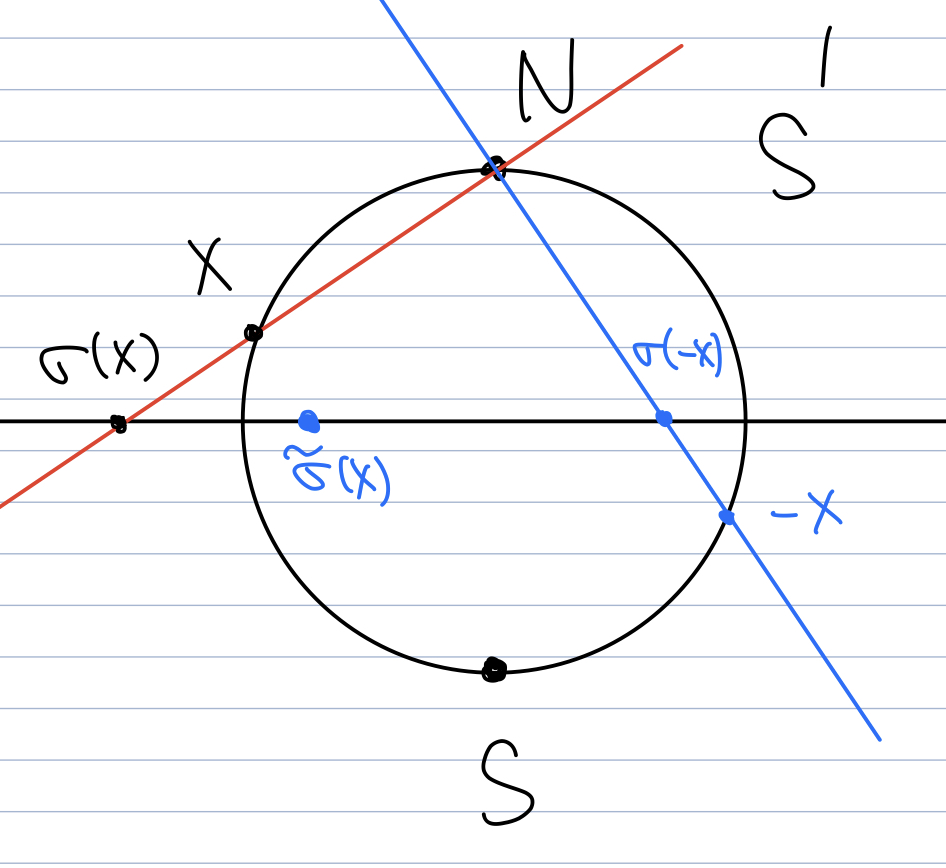
\includegraphics[width=.5\linewidth]{img/problem_1_7.jpeg}
    \caption{Problem 1-7}
    \label{fig:problem_1_7}
  \end{figure}
  $ $
  \begin{enumerate}[label=(\alph*)]
    \item 
      This is trivial from a basic trigonometry argument using the triangles $N, (0, \cdots, 0, x^{n + 1}), (x^1, \cdots, x^{n + 1})$ and $N, (0, \cdots, 0), \sigma(x^1, \cdots, x^{n + 1})$.
    \item
      $\sigma \circ \sigma^{-1}$ and $\sigma^{-1} \circ \sigma$ are both the identity maps, so $\sigma$ is bijective and $\sigma^{-1}$ is its inverse.
    \item
      Computation shows that $\tilde{\sigma} \circ \sigma^{-1}: S^n \setminus \{ N, S \} \rightarrow S^n \setminus \{ N, S \}$ sends $(u^1, \cdots, u^n)$ to $(u^1, \cdots, u^n) / \abs{u}^2$.
      As $\abs{u} \ne 0$ in the domain, this map is well-defined and clearly smooth.
      By Proposition 1.17(a), these two charts determine a unique smooth structure.
    \item
      $\phi_i, \sigma, \tilde{\sigma}$ are all smooth functions of subsets of Euclidean spaces, so transition maps are always smooth.
      By Proposition 1.17(b), the smooth structure determined by $\sigma, \tilde{\sigma}$ is the same as the one defined in Example 1.31.
  \end{enumerate}
\end{proof}

\begin{customprob}{1-12(Proof of Proposition 1.45)}
  Suppose $M_1, \cdots, M_k$ are smooth manifolds and $N$ is a smooth manifold with boundary.
  Then $M_1 \times \cdots \times M_k \times N$ is a smooth manifold with boundary, and $\partial (M_1 \times \cdots \times M_k \times N) = M_1 \times \cdots \times M_k \times \partial N$.
\end{customprob}

\begin{proof}
  By Example 1.34, $M_1 \times \cdots \times M_k$ is a smooth manifold.
  Thus it suffices to show that $M \times N$ is a smooth manifold with boundary if $M$ is a smooth manifold and $N$ is a smooth manifold with boundary.
  Let $m, n$ be the dimensions of $M, N$.

  First, we show that $M \times N$ is a topological manifold with boundary and $\partial(M \times N) = M \times \partial N$.
  Let $(p, q) \in M \times N$.
  Then $p \in M$, so there exists a chart $(U, \phi)$ such that $p \in U$ and $\hat{U} = \phi(U) \subset \mathbb{R}^m$.

  \begin{itemize}
    \item
      Suppose $q \in \Int N$.
      Then there exists a chart $(V, \psi)$ such that $\hat{V} = \psi(V) \subset \mathbb{R}^n$.
      $\phi \times \psi$ is a homeomorphism between $U \times V$ and $\hat{U} \times \hat{V} \subset \mathbb{R}^m \times \mathbb{R}^n = \mathbb{R}^{m + n}$.
      Thus $(U \times V, \phi \times \psi)$ is a chart for $(p, q)$.
    \item
      Suppose $q \in \bd N$.
      Then there exists a chart $(V, \psi)$ such that $\hat{V} = \psi(V) \subset \mathbb{H}^n$ and $\psi(q) \in \partial \mathbb{H}^n$.
      $\phi \times \psi$ is a homeomorphism between $U \times V$ and $\hat{U} \times \hat{V} \subset \mathbb{R}^m \times \mathbb{H}^n = \mathbb{H}^{m + n}$.
      Moreover, $(\phi \times \psi)(p, q) = (\phi(p), \psi(q)) \in \mathbb{R}^m \times \mathbb{H}^n = \mathbb{H}^{m + n}$.
      Thus $(U \times V, \phi \times \psi)$ is a boundary chart for $(p, q)$.
  \end{itemize}

  Therefore, $M \times N$ is a topological manifold with boundary and $\partial (M \times N) = M \times (\partial N)$.

  Let $\mathcal{A}_M, \mathcal{A}_N$ be the smooth structures of $M, N$.
  Define $\mathcal{A}_{M \times N} = \{ (U \times V, \phi \times \psi) \mid (U, \phi) \in \mathcal{A}_M, (V, \psi) \in \mathcal{A}_N \}$.
  Then $\mathcal{A}_{M \times N}$ is an atlas because we showed earlier that each $(U \times V, \phi \times \psi)$ is a chart.
  Let $(U_1 \times V_1, \phi_1 \times \psi_1), (U_2 \times V_2, \phi_2 \times \psi_2) \in \mathcal{A}_{M \times N}$.
  Then $(\phi_2 \times \psi_2) \circ (\phi_1 \times \psi_1)^{-1} = (\phi_2 \circ \phi_1^{-1}) \times (\psi_2 \circ \psi_1^{-1})$ is a smooth map from $(\phi_1 \times \psi_1)(U_1 \times V_1)$ into $(\phi_2 \times \psi_2)(U_2 \times V_2)$.
  Thus every pair of charts in $\mathcal{A}_{M \times N}$ is smoothly compatible.
  In other words, $\mathcal{A}_{M \times N}$ is a smooth atlas.

  On the other hand, $\mathcal{A}_{M \times N}$ must be maximal because the restriction of any smoothly compatible chart to $M, N$ gives a smoothly compatible chart, which must belong to $\mathcal{A}_M, \mathcal{A}_N$, respectively.
  Thus $M \times N$ is a smooth manifold with boundary.
\end{proof}


\end{document}


